\documentclass[12pt]{article}
\usepackage[utf8]{inputenc}
\usepackage{amsmath}
\usepackage{tocloft} 
\usepackage{hyperref}
\usepackage{graphicx}

\title{Explorando la Infraestructura Urbana. Una experiencia interactiva con cálculos de centralidad"}
\author{Jennifer de la C. Sánchez Santana\\ Reinaldo  Cánovas Gamón  }
\date{11 de Septiembre del 2024}

\begin{document}

\maketitle
\newpage

\tableofcontents
\newpage

\section{Introducción}

En el corazón de cada ciudad, en cada rincón del campo, se despliega una red de transporte vibrante y dinámica. Desde los autos que surcan las vías como flechas veloces, por ir al trabajo o regresar a casa, hasta los autobuses que serpentean por las calles, cada medio de transporte tiene su propio relato que contar. Pero, ¿qué sería de todos estos medios de transporte y las personas que se mueven en ellos si no existieran las carreteras?

Cada vez que te subes a uno de estos vehículos, no solo estás cambiando de lugar, sino que estás navegando por un vasto océano de conexiones invisibles. El transporte es más que solo el nombre; son ríos inmensos de información y tráfico continuo que van inundando nuestras vidas.

\section{Desarrollo}

\subsection{Las Redes de Transporte}

Las redes de transporte representan diferentes tipos de infraestructura \ o suministro de diversos modos. Las redes de carreteras y de tránsito son un medio principal para representar la oferta del transporte. Una red típica de autopistas incluiría enlaces desde alta velocidad y alta capacidad (por ejemplo, autopistas) hasta baja velocidad y baja capacidad (por ejemplo, calles o avenidas residenciales). Las redes de tránsito son una representación espacial de las rutas de autobús, ferrocarril y otros tipos de tránsito disponibles en una región.

Las redes de autopistas proporcionan una representación de enlaces individuales y conectados entre intersecciones a través del uso de enlaces y nodos. La red puede incluir miles de nodos y enlaces.

\subsection{Los Enlaces}

Los enlaces se describen a menudo por longitud, capacidad y número de carriles. Son elementos multifacéticos que van más allá de su función básica de conectar nodos. Influyen en la experiencia cotidiana de los usuarios, guían el desarrollo urbano, incorporan tecnologías avanzadas y, en algunos casos, adquieren un valor cultural e histórico significativo.

\subsection{Los Nodos}

Los nodos en una red de transporte son puntos cruciales que conectan múltiples enlaces, formando la base estructural del sistema. Son los puntos finales o iniciales de los trayectos, donde se dirige o se origina el tráfico. Estos son fundamentales para entender y analizar las redes de transporte, ya que determinan cómo se distribuye el tráfico y cómo se organizan los diferentes modos de transporte. Son los puntos centrales que dan forma y funcionalidad a las redes de transporte. Su diseño y gestión adecuadas son fundamentales para crear sistemas eficientes, sostenibles y que mejoren la calidad de vida de las comunidades. Representan intercambios, intersecciones señalizadas o sin señalizar, u otros puntos donde pueden tener lugar las transiciones en el tráfico.

\subsection{Centralidades}

Las centralidades son medidas matemáticas que revelan la importancia de cada nodo en una red de transporte. Estas medidas son cruciales para comprender la estructura y funcionamiento del sistema así como conocer qué intersecciones son más importantes en cuanto a mayor disponibilidad y rapidez en llegar a partir de esta a las demás.

Ejemplos de centralidades calculadas:

\begin{itemize}
    \item \textbf{Degree centrality} ayuda a identificar nodos altamente conectados, como intersecciones importantes o puntos de transferencia. Cuantifica el número de conexiones que tiene un nodo.
    \item \textbf{Closeness centrality} revela nodos que están más próximos a todos los demás, potencialmente actuando como centros de actividad. Es la medida de la distancia media más corta entre cada persona en una red.
    \item \textbf{Betweenness centrality} destaca nodos que controlan gran parte del tráfico, como cruces de carreteras principales. Es la medida de la frecuencia con la que un nodo se encuentra en el camino más corto entre todos los pares de nodos en una red.

\item \textbf{Eigenvector centrality} captura la influencia de los nodos en la red, ayudando a identificar puntos clave en la infraestructura urbana. Un nodo en un gráfico es más central si está conectado a otros nodos importantes.
    \item \textbf{Minimum Connected Time} mide la importancia de un nodo basada en el tiempo de conexión a otros nodos. Calcula la suma del tiempo de conexión a todos los demás nodos y la invierte.
\end{itemize}

Juntas, estas medidas proporcionan una vista amplia para la comprensión de la red de transporte, permitiendo analizar patrones de movilidad, identificar puntos críticos y optimizar la infraestructura urbana. En el ámbito de la sostenibilidad, conocer los nodos más importantes ayuda a optimizar la asignación de recursos y a implementar políticas de reducción de congestión.

\subsection{Nuestra Red}

En nuestra red interactiva es posible ajustar parámetros como las desviaciones que poseen las avenidas y calles, la cantidad de estas, las dimensiones de los carriles y cosas similares para que el usuario tenga una experiencia interactiva e interesante. Como también la posibilidad de eliminar aristas y nodos, simulando estancamientos o calles cerradas.\\


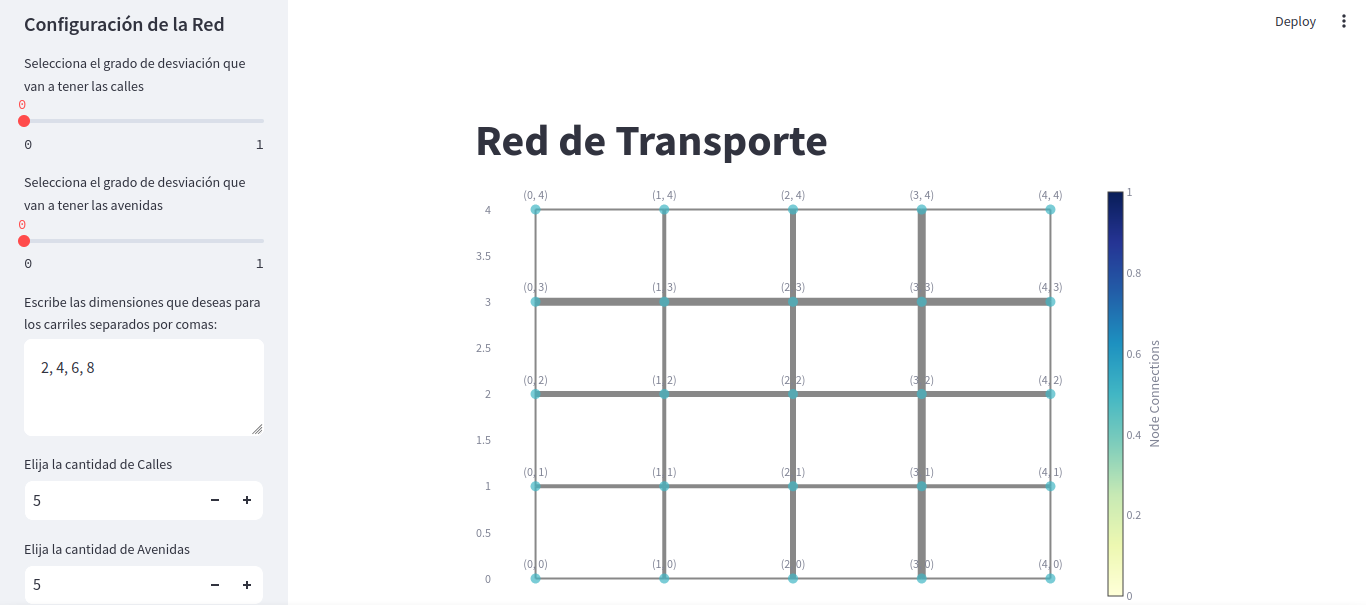
\includegraphics[scale=0.5]{imagen.png}

\section{Conclusiones}

La red de transporte es un sistema complejo y dinámico que influye profundamente en la vida cotidiana de las ciudades. El análisis de redes de transporte utilizando herramientas matemáticas como las centralidades nos permite entender mejor cómo funciona este sistema y cómo podemos mejorar su eficiencia y sostenibilidad. Es importante siempre identificar nodos clave y enlaces críticos, ya que esto es fundamental para entender la estructura básica de la red y tomar decisiones informadas sobre su mejora. Además, la necesidad de múltiples perspectivas es crucial, ya que las diferentes medidas de centralidad ofrecen visiones únicas del sistema, lo cual es indispensable para obtener una comprensión completa. La importancia de la interactividad también se hace evidente, ya que herramientas interactivas permiten a los usuarios experimentar y aprender sobre la red de manera práctica. Esta información es particularmente relevante para la planificación urbana, ya que el conocimiento obtenido a través del análisis de redes de transporte puede utilizarse para optimizar la infraestructura urbana, reducir la congestión y mejorar la calidad de vida de los ciudadanos. Finalmente, es fundamental considerar factores relacionados con la sostenibilidad ambiental y social al evaluar la importancia de los nodos y enlaces.

\section{Bibliografía}

\begin{itemize}
    \item Transportation networks.  \url{https://tfresource.org/topics/Transportation_networks.html}
    \item Highway networks. \url{https://tfresource.org/topics/Highway_networks.html}
    \item Centralidad. \url{https://www.grapheverywhere.com/centralidad/}
    \item Degree Centrality. \url{https://www.sciencedirect.com/topics/computer-science/degree-centrality}
    \item Closeness Centrality. \url{https://www.sciencedirect.com/topics/computer-science/closeness-centrality}
    \item Betweenness Centrality. \url{https://www.sciencedirect.com/topics/computer-science/betweenness-centrality}
    \item Eigenvector Centrality.  \url{https://www.sciencedirect.com/topics/computer-science/eigenvector-centrality}
    \item José Antonio de la Peña, EMALCA Team (2012). \textit{Sistemas de transporte en México: un análisis de centralidad en teoría de redes}.  \url{https://rde.inegi.org.mx/RDE_07/Doctos/RDE_07_Art6.pdf}
\end{itemize}


\end{document} 
